%% USPSC-Apendice.tex
% ---
% Inicia os apêndices
% ---

\begin{apendicesenv}
	% Imprime uma página indicando o início dos apêndices
	\partapendices
	\chapter{Additional tables of the textual differences found in all networks}\label{ap:textd}
In the following tables the counting of differences of textual features among the analyzed networks
are shown.
	These results are auxiliary for the discussion on Section~\ref{sec:tresults}.
\FloatBarrier
\begin{table}[h!]
\begin{center}
\caption{Counts of evidence of characters-related differences in the Erd\"os sectors in each of the analyzed networks.}
	\def\arraystretch{1.5}
\begin{tabular}{| l || c | c | c || c |}\hline
{\bf synset} & {\bf p.} & {\bf i.} & {\bf h} & {\bf peaks} \\\hline\hline
$\frac{spaces}{chars}$ & 2  & 0  & 8  & 2 \\
$\frac{punct}{chars-spaces}$ & 11  & 4  & 1  & 5 \\
$\frac{digits}{chars-spaces}$ & 9  & 7  & 2  & 10 \\\hline
$\frac{letters}{chars-spaces}$ & 0  & 0  & 3  & 0 \\
$\frac{vowels}{letters}$ & 0  & 1  & 1  & 1 \\
$\frac{uppercase}{letters}$ & 13  & 3  & 1  & 6 \\\hline
\end{tabular}
\begin{flushleft}
		Source: By the author.\
\end{flushleft}
\end{center}
\end{table}

\begin{table}[h!]
\begin{center}
\caption{Counts of evidence of token-related differences in the Erd\"os sectors in each of the analyzed networks.}
	\def\arraystretch{1.5}
\begin{tabular}{| l || c | c | c || c |}\hline
{\bf synset} & {\bf p.} & {\bf i.} & {\bf h} & {\bf peaks} \\\hline\hline
$\frac{knownw}{tokens}$ & 1  & 0  & 5  & 1 \\
$\frac{knownw \neq}{knownw}$ & 13  & 1  & 4  & 9 \\
$\frac{stopw}{knownw}$ & 0  & 0  & 14  & 2 \\
$\frac{punct}{tokens}$ & 10  & 3  & 1  & 3 \\
$\frac{contrac}{tokens}$ & 0  & 2  & 15  & 4 \\\hline
$\mu(\overline{tokens})$ & 0  & 1  & 2  & 1 \\
$\sigma(\overline{tokens})$ & 7  & 1  & 0  & 2 \\\hline
$\mu(\overline{knownw})$ & 0  & 0  & 2  & 0 \\
$\sigma(\overline{knownw})$ & 0  & 0  & 1  & 1 \\\hline
$\mu(\overline{knownw \neq})$ & 0  & 0  & 0  & 0 \\
$\sigma(\overline{knownw \neq})$ & 0  & 0  & 0  & 0 \\\hline
$\mu(\overline{stopw})$ & 0  & 0  & 0  & 0 \\
$\sigma(\overline{stopw})$ & 0  & 0  & 1  & 0 \\\hline
\end{tabular}
\begin{flushleft}
		Source: By the author.\
\end{flushleft}
\end{center}
\end{table}

\begin{table}[h!]
\begin{center}
\caption{Counts of evidence of sentence-related differences in the Erd\"os sectors in each of the analyzed networks.}
\begin{tabular}{| l || c | c | c || c |}\hline
{\bf synset} & {\bf p.} & {\bf i.} & {\bf h} & {\bf peaks} \\\hline\hline
$\mu_S(chars)$ & 9  & 3  & 1  & 6 \\
$\sigma_S(chars)$ & 11  & 6  & 1  & 9 \\\hline
$\mu_S(tokens)$ & 10  & 2  & 1  & 5 \\
$\sigma_S(tokens)$ & 9  & 7  & 1  & 9 \\\hline
$\mu_S(knownw)$ & 9  & 3  & 2  & 6 \\
$\sigma_S(knownw)$ & 11  & 5  & 2  & 8 \\\hline
$\mu_S(stopw)$ & 2  & 3  & 7  & 7 \\
$\sigma_S(stopw)$ & 6  & 7  & 4  & 10 \\\hline
$\mu_S(puncts)$ & 13  & 2  & 1  & 2 \\
$\sigma_S(puncts)$ & 7  & 8  & 1  & 8 \\\hline
\end{tabular}
\begin{flushleft}
		Source: Prepared by the authors.\
\end{flushleft}
\end{center}
\end{table}

\begin{table}[h!]
\begin{center}
\caption{Counts of evidence of message-related differences in the Erd\"os sectors in each of the analyzed networks.}
	\def\arraystretch{1.5}
\begin{tabular}{| l || c | c | c || c | c |}\hline
{\bf synset} & {\bf p.} & {\bf i.} & {\bf h} & {\bf peaks} & {\bf total} \\\hline\hline
$\mu_M(sents)$ & 4  & 7  & 1  & 9  & 16 \\
$\sigma_M(sents)$ & 5  & 7  & 2  & 11  & 15 \\\hline
$\mu_M(tokens)$ & 10  & 5  & 2  & 6  & 18 \\
$\sigma_M(tokens)$ & 8  & 8  & 2  & 9  & 18 \\\hline
$\mu_M(knownw)$ & 8  & 5  & 3  & 7  & 18 \\
$\sigma_M(knownw)$ & 10  & 5  & 3  & 9  & 18 \\\hline
$\mu_M(stopw)$ & 5  & 6  & 6  & 8  & 18 \\
$\sigma_M(stopw)$ & 7  & 6  & 3  & 11  & 18 \\\hline
$\mu_M(puncts)$ & 12  & 4  & 2  & 5  & 18 \\
$\sigma_M(puncts)$ & 8  & 9  & 1  & 10  & 18 \\\hline
$\mu_M(chars)$ & 10  & 5  & 2  & 6  & 18 \\
$\sigma_M(chars)$ & 9  & 7  & 2  & 8  & 18 \\\hline
\end{tabular}
\begin{flushleft}
		Source: Prepared by the authors.\
\end{flushleft}
\end{center}
\end{table}

\begin{table}[h!]
\begin{center}
\caption{Counts of evidence of differences related to POS tags in the Erd\"os sectors in each of the analyzed networks.}
\begin{tabular}{| l || c | c | c || c |}\hline
{\bf synset} & {\bf p.} & {\bf i.} & {\bf h} & {\bf peaks} \\\hline\hline
NOUN & 13  & 1  & 0  & 1 \\
X & 4  & 9  & 5  & 14 \\\hline
ADP & 0  & 1  & 4  & 1 \\
DET & 1  & 0  & 9  & 2 \\\hline
VERB & 0  & 0  & 6  & 1 \\\hline
ADJ & 1  & 2  & 6  & 2 \\
ADV & 0  & 0  & 17  & 1 \\\hline
PRT & 1  & 1  & 9  & 4 \\
PRON & 0  & 1  & 11  & 3 \\
NUM & 8  & 5  & 3  & 7 \\
CONJ & 2  & 6  & 4  & 8 \\\hline
\end{tabular}
\begin{flushleft}
		Source: By the author.\
\end{flushleft}
\end{center}
\end{table}

\begin{table}[h!]
\begin{center}
\caption{Counts of evidence of differences related to Wordnet POS tags in the Erd\"os sectors in each of the analyzed networks.}
\begin{tabular}{l || c | c | c || c}\hline
{\bf synset} & {\bf p.} & {\bf i.} & {\bf h} & {\bf peaks} \\\hline\hline
N & 8  & 1  & 0  & 1 \\
ADJ & 0  & 2  & 12  & 6 \\
VERB & 0  & 1  & 16  & 2 \\
ADV & 0  & 0  & 9  & 1 \\\hline\hline
POS & 0  & 0  & 3  & 1 \\
POS! & 0  & 1  & 0  & 1 \\\hline
\end{tabular}
\begin{flushleft}\footnotesize
		Source: By the author.\
\end{flushleft}
\end{center}
\end{table}

\begin{table}[h!]
\begin{center}
\caption{Counts of evidence of differences related to Wordnet noun synset characteristics in the Erd\"os sectors in each of the analyzed networks.}
\begin{tabular}{| l || c | c | c || c |}\hline
{\bf synset} & {\bf p.} & {\bf i.} & {\bf h} & {\bf peaks} \\\hline\hline
$\mu(min\,depth)$ & 0  & 0  & 0  & 0 \\
$\sigma(min\,depth)$ & 1  & 1  & 2  & 1 \\\hline
$\mu(max\,depth)$ & 0  & 0  & 0  & 0 \\
$\sigma(max\,depth)$ & 0  & 1  & 3  & 1 \\\hline
$\mu(holonyms)$ & 7  & 4  & 4  & 6 \\
$\sigma(holonyms)$ & 3  & 4  & 7  & 6 \\\hline
$\mu(meronyms)$ & 8  & 5  & 3  & 7 \\
$\sigma(meronyms)$ & 12  & 4  & 2  & 9 \\\hline
$\mu(domains)$ & 6  & 4  & 5  & 8 \\
$\sigma(domains)$ & 3  & 1  & 4  & 3 \\\hline
$\mu(lemmas)$ & 6  & 0  & 1  & 2 \\
$\sigma(lemmas)$ & 6  & 2  & 2  & 4 \\\hline
$\mu(hyponyms)$ & 1  & 6  & 6  & 9 \\
$\sigma(hyponyms)$ & 4  & 6  & 6  & 11 \\\hline
$\mu(hypernyms)$ & 0  & 0  & 0  & 0 \\
$\sigma(hypernyms)$ & 4  & 4  & 4  & 6 \\\hline
\end{tabular}
\begin{flushleft}
		Source: Prepared by the authors.\
\end{flushleft}
\end{center}
\end{table}

\begin{table}[h!]
\begin{center}
\caption{Counts of evidence of differences related to Wordnet adjective synset characteristics in the Erd\"os sectors in each of the analyzed networks.}
\begin{tabular}{| l || c | c | c || c |}\hline
{\bf synset} & {\bf p.} & {\bf i.} & {\bf h} & {\bf peaks} \\\hline\hline
$\mu(domains)$ & 2  & 6  & 8  & 10 \\
$\sigma(domains)$ & 2  & 4  & 5  & 7 \\\hline
$\mu(similar)$ & 1  & 0  & 7  & 4 \\
$\sigma(similar)$ & 4  & 0  & 5  & 3 \\\hline
$\mu(lemmas)$ & 1  & 2  & 1  & 2 \\
$\sigma(lemmas)$ & 6  & 3  & 4  & 6 \\\hline
\end{tabular}
\begin{flushleft}
		Source: By the author.\
\end{flushleft}
\end{center}
\end{table}

\begin{table}[h!]
\begin{center}
\caption{Counts of evidence of differences related to Wordnet verb synset characteristics in the Erd\"os sectors in each of the analyzed networks.}
\begin{tabular}{| l || c | c | c || c |}\hline
{\bf synset} & {\bf p.} & {\bf i.} & {\bf h} & {\bf peaks} \\\hline\hline
$\mu(min\,depth)$ & 2  & 1  & 1  & 3 \\
$\sigma(min\,depth)$ & 2  & 1  & 1  & 2 \\\hline
$\mu(max\,depth)$ & 2  & 1  & 0  & 1 \\
$\sigma(max\,depth)$ & 3  & 1  & 1  & 2 \\\hline
$\mu(domains)$ & 7  & 3  & 4  & 4 \\
$\sigma(domains)$ & 8  & 3  & 3  & 5 \\\hline
$\mu(verb\,groups)$ & 0  & 2  & 3  & 2 \\
$\sigma(verb\,groups)$ & 0  & 0  & 0  & 0 \\\hline
$\mu(lemmas)$ & 0  & 0  & 2  & 0 \\
$\sigma(lemmas)$ & 1  & 0  & 3  & 0 \\\hline
$\mu(entailments)$ & 7  & 1  & 7  & 3 \\
$\sigma(entailments)$ & 4  & 1  & 5  & 3 \\\hline
$\mu(hyponyms)$ & 1  & 2  & 6  & 3 \\
$\sigma(hyponyms)$ & 2  & 3  & 8  & 6 \\\hline
$\mu(hypernyms)$ & 2  & 2  & 0  & 2 \\
$\sigma(hypernyms)$ & 1  & 0  & 1  & 1 \\\hline
\end{tabular}
\begin{flushleft}
		Source: By the author.\
\end{flushleft}
\end{center}
\end{table}

\begin{table}[h!]
\begin{center}
\caption{Counts of evidence of differences related to Wordnet adverb synset characteristics in the Erd\"os sectors in each of the analyzed networks.}
\begin{tabular}{| l || c | c | c || c |}\hline
{\bf synset} & {\bf p.} & {\bf i.} & {\bf h} & {\bf peaks} \\\hline\hline
$\mu(domains)$ & 3  & 3  & 10  & 10 \\
$\sigma(domains)$ & 1  & 4  & 7  & 7 \\\hline
$\mu(lemmas)$ & 0  & 0  & 1  & 1 \\
$\sigma(lemmas)$ & 3  & 1  & 2  & 4 \\\hline
\end{tabular}
\begin{flushleft}
		Source: Prepared by the authors.\
\end{flushleft}
\end{center}
\end{table}


\chapter{Developments made in this research but not included elsewhere in this thesis}\label{ap:vot}
In this appendix are gathered developments relevant for the initial proposal of this research:
enabling the use of complex networks scientific knowledge by the participant of the social networks.
These developments are not included elsewhere in the thesis because we chose to present results
more closely related to physics in a simple fashion.
Furthermore, most of the following contributions have received dedicated documentation,
reason why we next only summarize and cite the documents when they are available.

\section{Continuous voting by approval and participation}
In finding the adequate way to prioritize proposals, the Brazilian social participation community agreed about the measurement of two indexes,
one of approval and one of participation. Both practice and literature
was constantly handled by the experts involved, and the formalization
of such model and metrics and is very simple and seems novel.
Also, the relevance of this development is strengthened by the use of these indexes by the
Brazilian General Secretariat of the Republic to raise and prioritize
proposals about public health care in open processes.
This was achieved by means of the Dialoga Brasil federal platform~\cite{dialoga}.
A short report on these indexes and their use is on~\cite{dialogaAlg}
	(co-authorship by Ricardo Poppi).

	\section{Visualization of static networks}
	In Sections~\ref{sec:versinus0} and~\ref{sec:versinus1} we addressed a visualization method of networks through animations.
	We also made many static network visualizations which were important for our research.
	Many of these were made by testing software and programming libraries.
	We next exemplify such efforts by probably the most important and time-consuming realizations.

	\subsection{Static email networks visualization using Networkx and Graphviz and a PHP web interface}\label{sec:autoRede}
	At the start of this research, we observed many networks derived from email lists
	by means of a web interface we wrote.
	In such web interface, which was accessed as a usual webpage through HTTP in a web browser, 
	the user could specify an email list, start and end messages and a window size (number of messages taken together to obtain the network).
	The interface then rendered graph visualizations and standard measures such as degree, strength, clustering coefficient, betweenness centrality, both as histograms and as mean and standard deviation.
	In the node-link diagrams, measurements were mapped to height, width and color of nodes and to link characteristics.
	The software source code is available in~\cite{autoRede} and an example image is Figure~\ref{fig:autoRede}.
\begin{figure}[h!]
\begin{center}
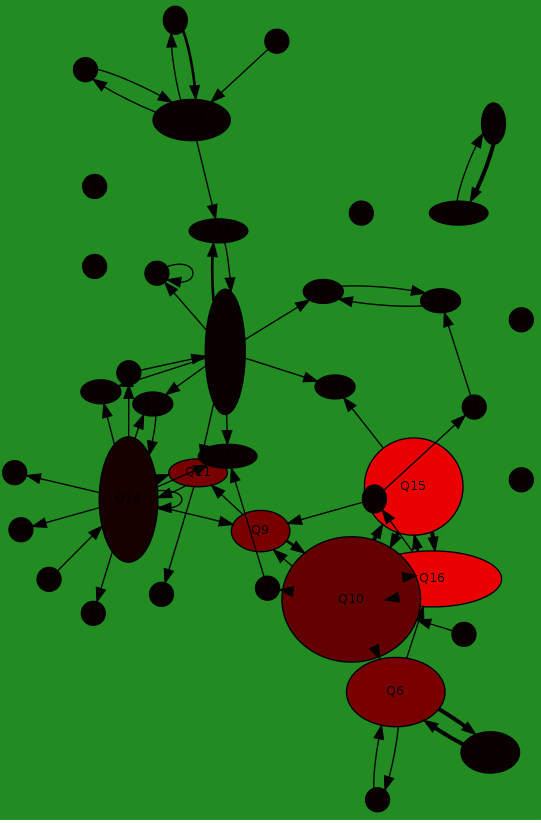
\includegraphics[scale=.25]{figs/autoRede_}
\caption{An example image rendered from the first online gadget made in this research for studying social networks.
	The app also delivered measurements, 2D plots and GML graph files. For further information please see Section~\ref{sec:autoRede}}
\label{fig:autoRede}
\begin{flushleft}\footnotesize
Source: By the author.\
\end{flushleft}
\end{center}
\end{figure}
% email pelo app online

	\subsection{Static Facebook networks visualization using Gephi}\label{sec:gephi}
	Mainly in the years of 2013 and 2014, Facebook users retrieved their friendship networks through Netvizz software~\cite{netvizz}
	and donated them to our research.
	I also retrieved friendship and interaction networks from Facebook groups I was a member, also using Netvizz.
	These networks were used for information collection and diffusion (explained in Section~\ref{sec:colDif}),
	taking measurements and visualization.
	The visualizations were achieved almost exclusively through the Gephi software~\cite{gephi}
	and is included in this appendix for being used a number of times by fellow researchers and artists.
	The most useful layout algorithm was Force Atlas 2~\cite{fa2} and an example of these images is Figure~\ref{fig:gephi}.

% \begin{figure}[h!]
% \begin{center}
% 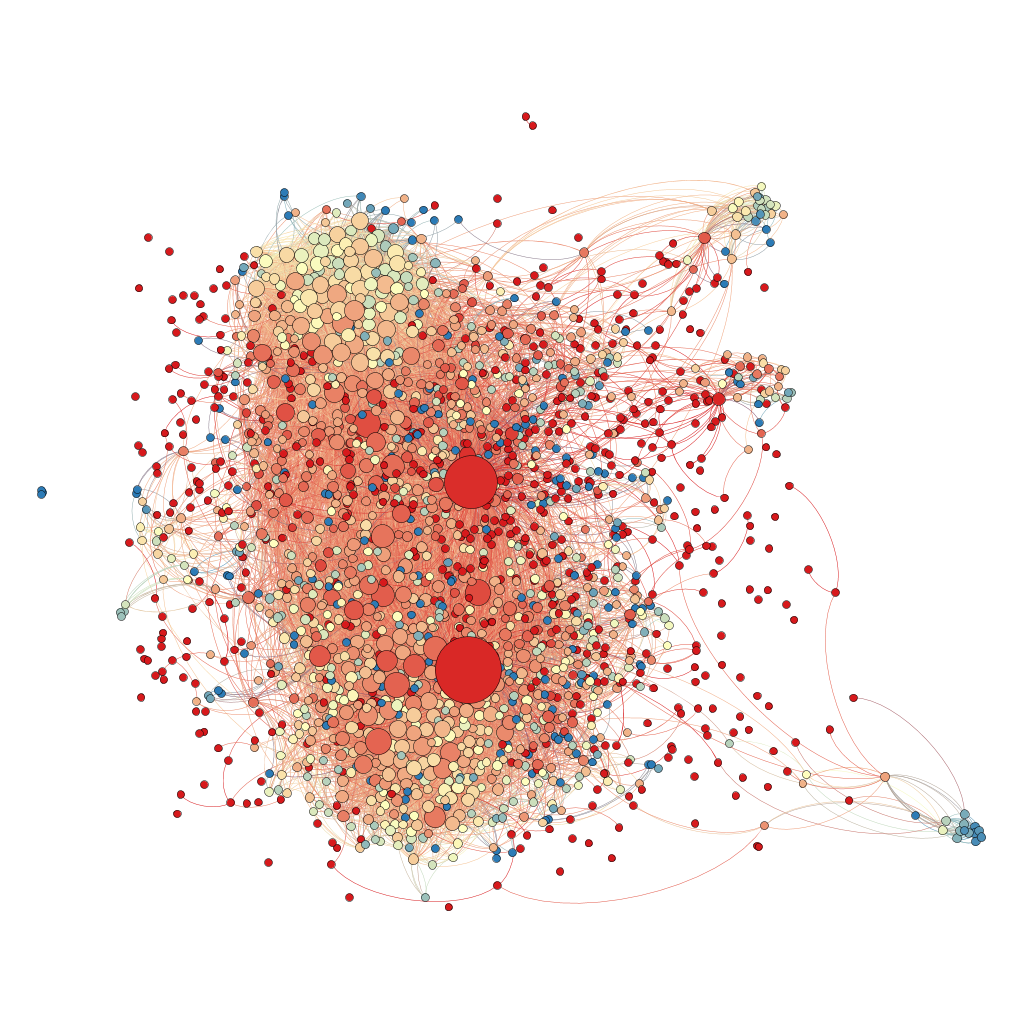
\includegraphics[scale=.25]{figs/Silicon}
% 	\caption{An example network image rendered from the Silicon Valley (Facebook) group using Gephi and the Force Atlas 2 layout algorithm.
% 	See Section~\ref{sec:gephi} for further information.}
% \label{fig:gephi}
% \begin{flushleft}\footnotesize
% Source: By the author.\
% \end{flushleft}
% \end{center}
% \end{figure}

\begin{figure}[!tbp]
	\centering
	    \subfloat[\footnotesize Without participant names.]{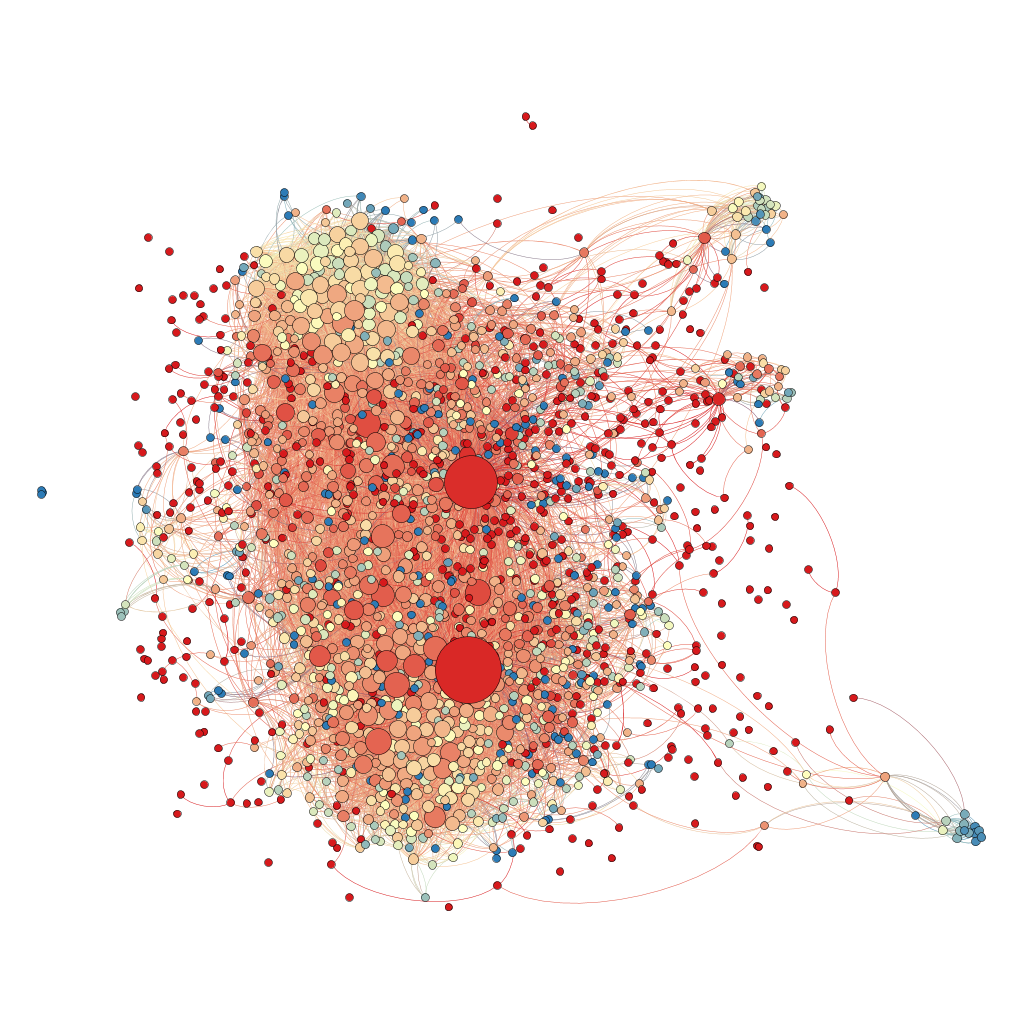
\includegraphics[width=0.45\textwidth]{figs/Silicon.png}\label{fig:f1}}
		\subfloat[\footnotesize With participant names.]{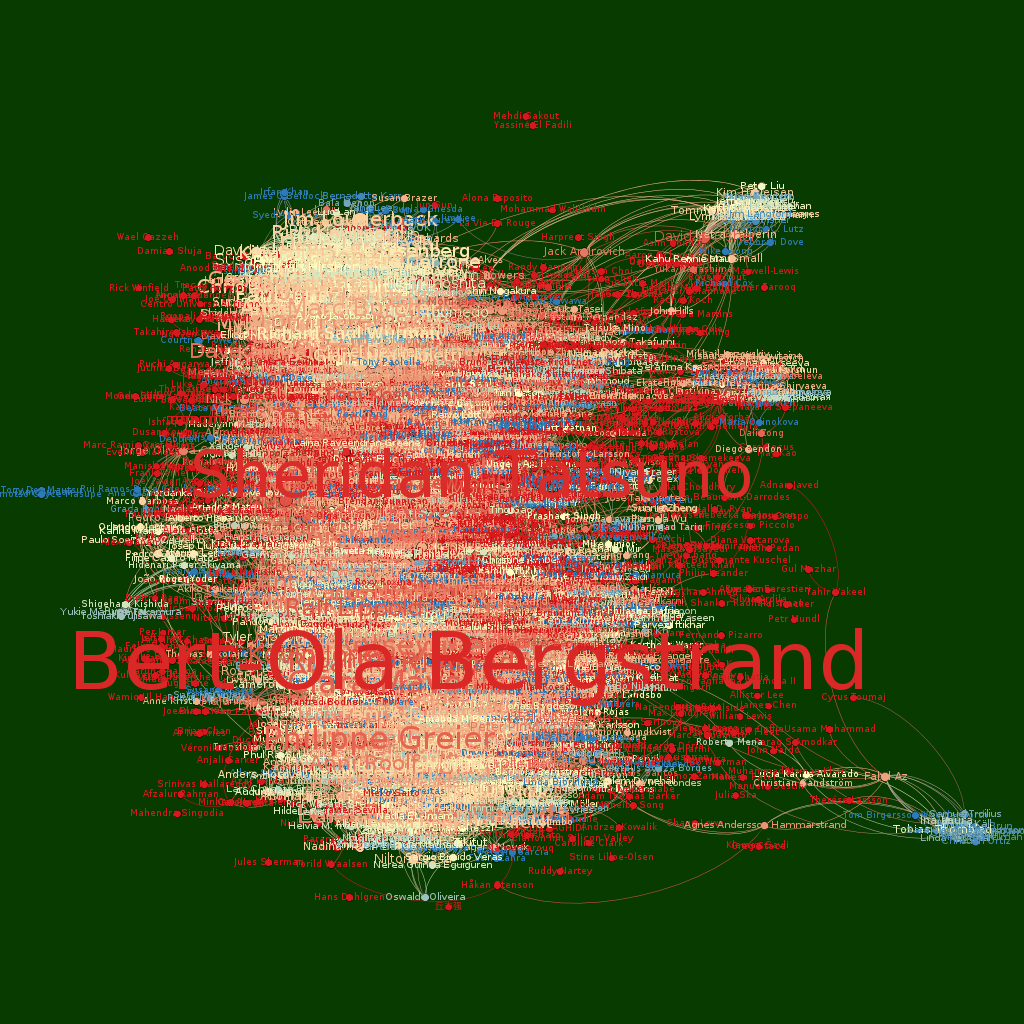
\includegraphics[width=0.45\textwidth]{figs/Silicon_nomes.png}\label{fig:f2}}
	\caption{An example network image rendered from the Silicon Valley (Facebook) group using Gephi and the Force Atlas 2 layout algorithm.
	See Section~\ref{sec:gephi} for further information.}\label{fig:gephi}
\begin{flushleft}\footnotesize
Source: By the author.\
\end{flushleft}
\end{figure}

	\subsection{Art by Pedro Paulo Rocha}\label{sec:ppr}
	The static images rendered for the visualization of networks were at time also used for artistic elaborations.
	Apart from other artistic incidences reported in this appendix (such as in Sections~\ref{sec:govArt} and~\ref{sec:soundSkull})
	we present in Figure~\ref{fig:ppr} an example art from Pedro Paulo Rocha.
	More of his work that is derived from our network visualizations are gathered in an image Gallery~\cite{pprGal}.
\begin{figure}[h!]
\begin{center}
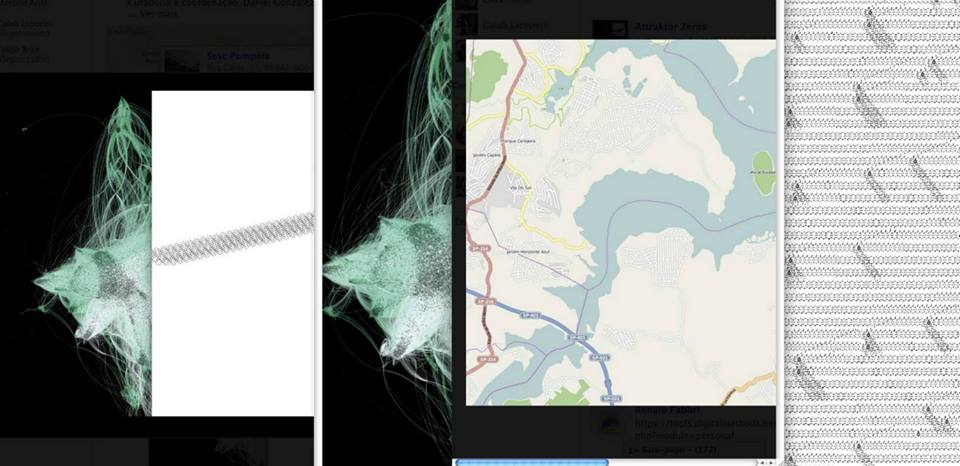
\includegraphics[scale=.45]{figs/ppr}
\caption{An example artistic image by Pedro Paulo Rocha and derived from our network visualizations.
	For further information please see Section~\ref{sec:ppr}}
\label{fig:ppr}
\begin{flushleft}\footnotesize
Source: Provided by the artist Pedro Paulo Rocha. Image derived from other images by the author.\
\end{flushleft}
\end{center}
\end{figure}

\section{Mega networks}\label{sec:megarrede}
The most usual social networking platform nowadays is Facebook.
In this platform, one cannot have more than 5000 friends.
To analyze larger friendship network social structure through Facebook,
we started merging the networks from distinct users.
From this procedure we obtained networks with tenths of thousands of participants
and even a few which reached the scale of hundreds of thousands.
Such practice started at AVLAB 6 in SESC Pompéia (directed by Daniel Gonzales Xavier)
and was further developed in a number of occasions by us and other researchers.
Figure~\ref{fig:megarrede} exemplifies one of such structures.
\begin{figure}[h!]
\begin{center}
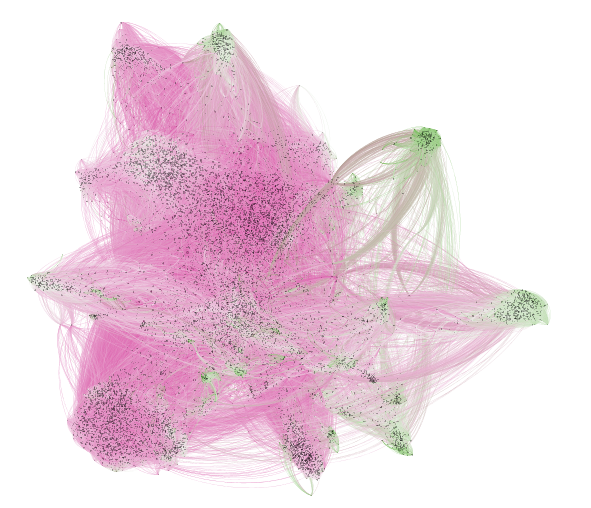
\includegraphics[scale=.45]{figs/megarrede}
\caption{An example visualization of a mega network with tenths of thousands of participants derived from Facebook ego networks.
	For further information please see Section~\ref{sec:megarrede}}
\label{fig:megarrede}
\begin{flushleft}\footnotesize
Source: By the author.\
\end{flushleft}
\end{center}
\end{figure}
% arte pelo Pedro Paulo Rocha

\section{Social structures live streaming (networks and language-related)}\label{sec:sss}
A strong trait I could observe with the cycles of information gathering and diffusion (see Section~\ref{sec:clDif})
is the timid appropriation of the social structures by their participants.
Some people are enchanted by the figures,
others by the concepts and by the perception of the social aspect of themselves,
sometimes called ``network being'' or `` I-network '' by interested parties during the broadcasts.
In these contexts, academic theories, such as the Network Actor Theory (Latour),
were rarely recalled directly, even by specialists.
The efficiency of the intuitive discourse to communicate about these interests is impressive.
The impulse to report the impressions resembles the urge to report dreams,
with glimpses of subtle and unconscious structures and sequential forgetfulness.
In this context, in order to spread about how our traces can be observed and taken advantage of,
we programmed screens of social structures streaming in HTML pages.
Only Twitter was used, and networks yield by retweets,vocabulary and hashtags were contemplated.
The screen could also display recent tweets, more occurring words, co-occurrences,
and other simple text information.
These screens were used e.g. in the Arena NET Mundial event
and in mobilizations such as the one identified with the \#ocupaGOV hashtag.
Figures~\ref{fig:telao1} and~\ref{fig:telao2} exemplify such interfaces.
They were updated live as tweets were sent by all Twitter users whose messages
contained the selected hashtags.
The source code is publicly available in~\cite{teloes}.

\begin{figure}[H]
  \centering
    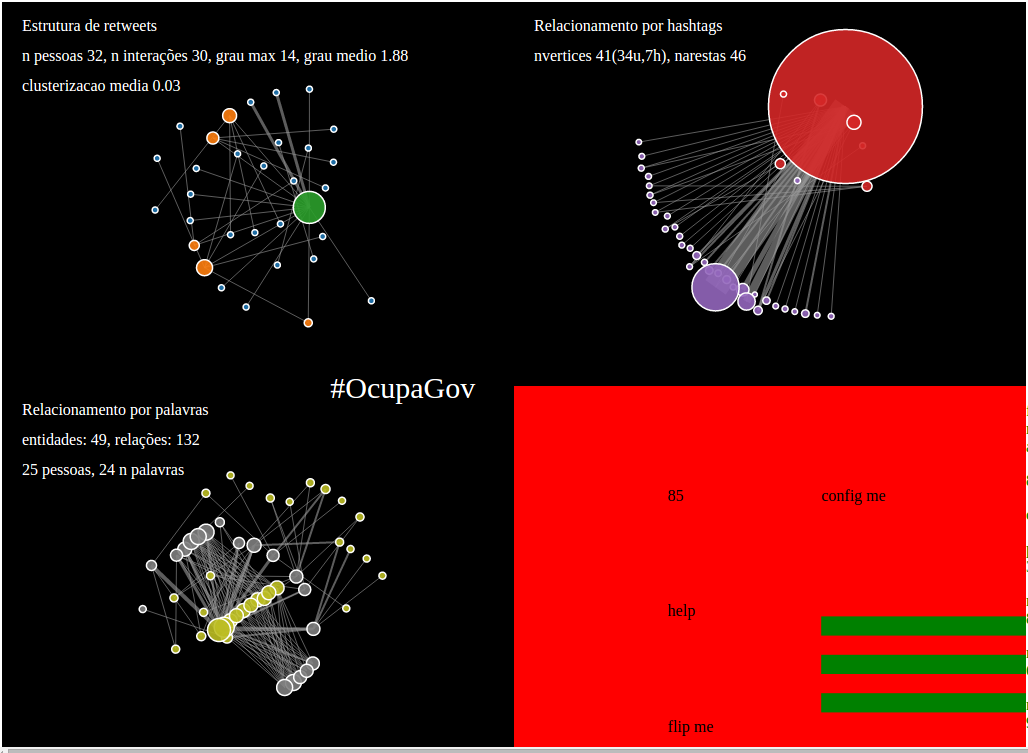
\includegraphics[width=.85\textwidth]{figs/telao1.png}
  \caption{Network interfaces of the live social structures streaming gadgets we programmed.
	Further information is on Section~\ref{sec:sss}.}\label{fig:telao1}
\end{figure}

\begin{figure}[H]
  \centering
    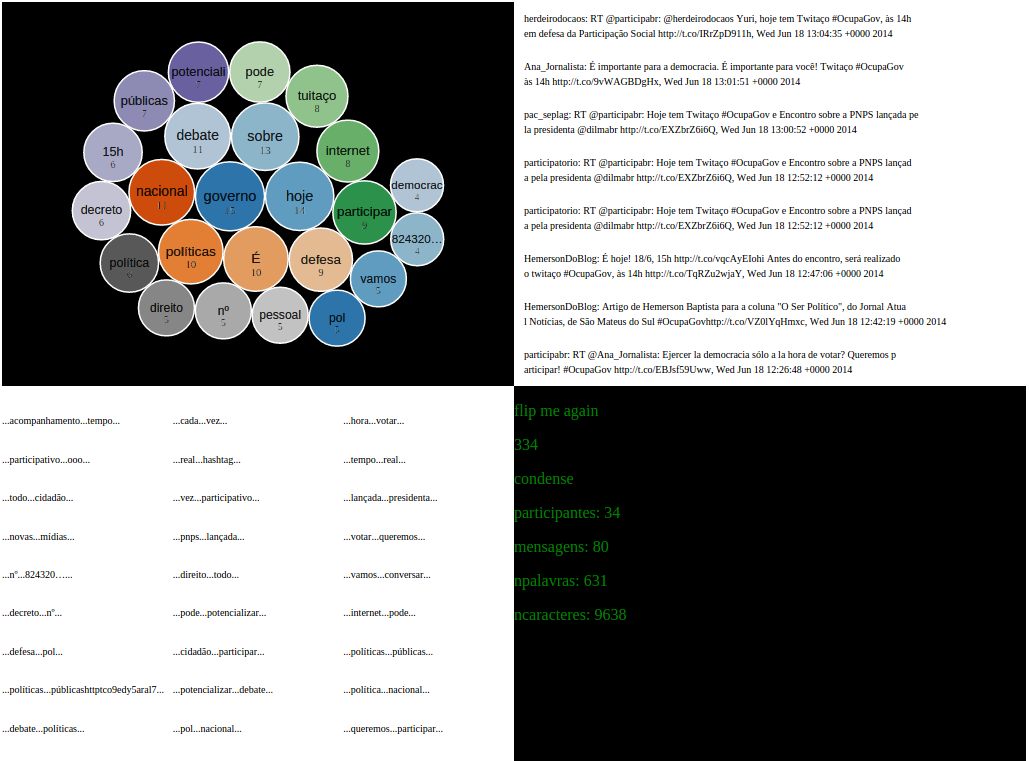
\includegraphics[width=.85\textwidth]{figs/telao2.png}
  \caption{Language-related interfaces of the live social structures streaming gadgets we programmed.
	Further information is on Section~\ref{sec:sss}.}\label{fig:telao2}
\end{figure}
\section{Ubiquity of inequality: a simple model that explains why power laws are so frequently found in empirical data}
% telões de redes e de medidas de texto
% uso no arenaNETmundial e no ocupaGOV e outras ocasiões online
\section{Kolmogorov-Smirnov test systematic measurements}
\section{OPS: the Social Participation (OWL) Ontology}
\section{OPa: the ParticipaBR (OWL) Ontology}
\section{OntologiAA: the AA (OWL) Ontology}
\section{The Algorithmic Autoregulation software development methodology}
\section{Social Library Ontology and Social Library Vocabulary: OBS in OWL and VBS in SKOS}
% Conselhos, Foruns, Mesas Redondas, etc. Casos feitos com especialistas, casos feitos a partir de documentações
\section{Genesis of this work: complex social networks analysis by emails}
\section{United Nations Development Program consulting}
\subsection{Partnership with the Brazilian Presidency}
\subsection{Description of each product}
\section{Govern art}\label{sec:govArt}
\section{Sounding Skull: a Rilke proposed transcendental experiment}\label{sec:soundSkull}
\section{Ideal ideas: a physical modeling of the mind}
\section{Webpages}
% ARS, texto para pedro
\section{Collection and diffusion of information in social networks}\label{sec:colDif}
\subsection{Progressive network activation from peripherals to hubs}
\subsection{Instantaneous network activation by betweenness and closeness centralities}
\subsection{Massive tagging in Facebook and email crossposting}
\subsection{SERVDDCR online video conferences}
% processo dos periféricos aos hubs
% instantâneos pelos de maior betweenness e maior closeness
% coleta e difusão através da citação de várias pessoas e de crosspost
% SERVDDCR
\section{Anthropological physics}
The study of complex systems can be undertaken as a physics endeavor,
specially if complex networks and statistics are into play. When the complex
system is constituted by people, intriguing questions arise from diverse field such as math, ethics, and sociology. The “anthropological physics”is an approach to these scenarios that enables scientific research while resolving ethical and moral issues by an open study of the self.
	It yields a transdisciplinary practice whose relevance emanate from anthropological
and physical matters, from human constituted systems and natural laws.
A sweet spot was found in recent civil, government and academic efforts~\cite{opa,ensaio}, and has been called anthropological physics. General characteristics are:
\begin{itemize}
	\item Exposure of the researcher to the environment of interest, such as virtual social networks.
	\item Use of the annotations from the exposure, be them activity logs, friendship or interaction networks, textual contents, etc.
	\item Upon need, expansion of observations to encompass open datasets or data donated by partners.
	\item Observance of natural laws as they appear in network structures and natural language.
	\item All resources are kept as open and publicized as possible, including software, data, and writings.
\end{itemize}                                                                                                                                     
A short report the first insights regarding anthropological physics is on~\cite{anPhy}.
 
% conceitualização básica, artigo e conferências
\section{Listing of documents written, conferences attended and artistic presentations}
% rcpln
% artigos
% conferências: duas nexos+ccdc+linguística+sifiscs+ufpa+
% apresentações na SGPR, imersões, arenaNETmundial
% vivace

\end{apendicesenv}
